% =========================================================================
%  Habeas Protocol -- arXiv submission
%  Compile with:  pdflatex main.tex && pdflatex main.tex
%  (two passes to resolve \ref / hyperref / TOC if needed)
% =========================================================================

\documentclass[11pt,letterpaper]{article}

% --- typography & layout -------------------------------------------------
\usepackage[T1]{fontenc}
\usepackage[utf8]{inputenc}
\usepackage{lmodern}
\usepackage{microtype}
\usepackage[letterpaper,top=1in,bottom=1in,left=1.15in,right=1.15in]{geometry}
\usepackage{setspace}
\setstretch{1.08}
\usepackage{enumitem}
\setlist[itemize]{itemsep=2pt,topsep=4pt}
\setlist[enumerate]{itemsep=2pt,topsep=4pt}

% --- math / symbols ------------------------------------------------------
\usepackage{amsmath,amssymb}

% --- color palette -------------------------------------------------------
\usepackage[dvipsnames,table]{xcolor}
\definecolor{ink}{HTML}{1A1A1A}
\definecolor{ink2}{HTML}{4A4A4A}
\definecolor{rule}{HTML}{D8D6CF}
\definecolor{accent}{HTML}{0F4C5C}
\definecolor{difc}{HTML}{C44536}
\definecolor{adgm}{HTML}{2C6E49}
\definecolor{sicc}{HTML}{8C5E3C}
\definecolor{good}{HTML}{2C6E49}
\definecolor{bad}{HTML}{B23A48}
\definecolor{paper}{HTML}{F8F5EE}
\definecolor{paper2}{HTML}{F0EDE5}

% --- section headings ----------------------------------------------------
\usepackage[explicit]{titlesec}
\titleformat{\section}{\normalfont\bfseries\large\color{accent}}{\thesection}{0.7em}{#1}
\titleformat{\subsection}{\normalfont\bfseries\normalsize\color{ink}}{\thesubsection}{0.6em}{#1}
\titleformat{\subsubsection}{\normalfont\itshape\normalsize\color{ink2}}{\thesubsubsection}{0.5em}{#1}
\titlespacing*{\section}{0pt}{18pt}{6pt}
\titlespacing*{\subsection}{0pt}{12pt}{4pt}

% --- tables --------------------------------------------------------------
\usepackage{booktabs}
\usepackage{array}
\newcolumntype{R}{>{\raggedleft\arraybackslash}p{0.06\textwidth}}
\newcolumntype{L}{>{\raggedright\arraybackslash}p{0.18\textwidth}}
\renewcommand{\arraystretch}{1.18}

% --- callouts ------------------------------------------------------------
\usepackage[framemethod=TikZ]{mdframed}
\newmdenv[
  linecolor=accent,
  linewidth=0pt,
  leftline=true,
  innerleftmargin=12pt,
  innertopmargin=8pt,
  innerbottommargin=8pt,
  innerrightmargin=8pt,
  backgroundcolor=paper2,
  skipabove=8pt,
  skipbelow=8pt
]{callout}

% --- figures -------------------------------------------------------------
\usepackage{tikz}
\usepackage{pgfplots}
\pgfplotsset{compat=1.18}
\usetikzlibrary{positioning,arrows.meta,shapes,calc,decorations.pathreplacing,backgrounds,fit}

% --- hyperref last -------------------------------------------------------
\usepackage[colorlinks=true,urlcolor=accent,linkcolor=accent,citecolor=accent]{hyperref}
\hypersetup{
  pdftitle={Habeas Protocol: A Computational-Legitimacy Framework for Digital-Jurisdiction Commercial Tribunals},
  pdfauthor={Hamza Qureshi},
  pdfsubject={Computational law; legal informatics; formal methods; arbitration},
  pdfkeywords={computational law, Catala, DIFC, ADGM, SICC, New York Convention, digital jurisdiction, FinTech regulation, formal methods, legal informatics},
  pdfproducer={pdfLaTeX},
  pdflang={en-US}
}

% --- title block ---------------------------------------------------------
\title{
  \vspace{-2em}
  \LARGE\bfseries\color{ink}
  Habeas Protocol\\[0.4em]
  \large\normalfont\color{ink2}
  A Computational-Legitimacy Framework for Digital-Jurisdiction\\
  Commercial Tribunals: Evidence from DIFC, ADGM, and SICC
}
\author{
  Hamza Qureshi\\
  \small Maxim Labs\\
  \small \texttt{thehamzaq@gmail.com}\\
  \small \href{https://github.com/thehamzaq/habeas-protocol}{\texttt{github.com/thehamzaq/habeas-protocol}}
}
\date{May 2026}

% =========================================================================
\begin{document}
\maketitle

% --- abstract ------------------------------------------------------------
\begin{callout}
\noindent\textbf{Abstract.}
Most proposals for handling cross-border digital-commerce disputes propose to invent a new tribunal -- a ``Web3 court,'' a metaverse arbitration body, a DAO-native dispute layer. This paper inverts that framing: \textbf{the tribunals already exist; what is missing is the computational layer.} We code 121 publicly-issued judgments from three operating special-jurisdiction commercial courts -- the Dubai International Financial Centre (DIFC) Courts, the Abu Dhabi Global Market (ADGM) Courts, and the Singapore International Commercial Court (SICC) -- against six per-ruling primitives a digital tribunal must satisfy and two architectural system properties. All three score at near-ceiling: SICC averages \textbf{1.95\,/\,2.00}, ADGM \textbf{1.91}, DIFC \textbf{1.72}. The pattern survives a 10$\times$ ADGM sample expansion (1.93 $\to$ 1.91) and replicates on a third tribunal in a different legal family. All three score 2/2 on both system properties. We then compile \textbf{seven rules} from the corpus into Catala source plus a Python predicate evaluator, demonstrating coverage of (i) static formulae, (ii) deferred conditionals, (iii) bounded discretion, (iv) arithmetic composition over substantive findings, (v) Boolean composition over contractual interpretation, (vi) partial New York Convention refusal under Singapore IAA s 31, and (vii) a third-party-jurisdiction disclosure gate over a USD 456M stablecoin tracing dispute. The protocol reproduces the courts' principal outputs exactly in six of seven traces; in the seventh it bounds a discretion residue at $\approx$ 6.92\% of the claim. Three traces surface clerical or methodological gaps in the courts' published orders. The constructive contribution is a 12-module open-source rule library, a 17-endpoint API, and a public dashboard, all running under continuous integration with 744 property-test invariants. Code: MIT. Data: CC BY 4.0.
\end{callout}

\vspace{0.5em}
\noindent\small\textit{Keywords:} computational law, legal informatics, formal methods, Catala, DIFC, ADGM, SICC, New York Convention, digital jurisdiction, FinTech regulation.

\smallskip
\noindent\small\textit{ACM CCS:} Applied computing $\to$ Law; Software and its engineering $\to$ Domain specific languages; Theory of computation $\to$ Logic and verification.

\smallskip
\noindent\small\textit{Funding and conflicts of interest:} This work received no external funding. The author declares no conflicts of interest. All artefacts are released under permissive open-source licences (MIT for code, CC BY 4.0 for data).

% =========================================================================
\section{Introduction}
% =========================================================================

In April 2024, Roblox Corporation faced its 31st child-safety lawsuit in twelve months. By 2025 the count had crossed 47, consolidated into multidistrict litigation. The substance was uniformly horrifying. The procedural posture was conventional: state and federal courts, plaintiffs' bar, common-law negligence pleadings, no novel forum, no novel doctrine. A digital-platform problem of historic scale had been routed entirely through the existing court system.

This paper begins with that observation because it complicates the dominant framing in the ``law for digital worlds'' literature. The literature presumes a missing tribunal: that as digital commerce scales, the legal infrastructure of the physical world becomes structurally inadequate, and a new dispute-resolution body must be designed and stood up. The Roblox case is one of many that contradicts the premise empirically. The legal infrastructure routes the disputes. What it does not yet do is route them \textit{computationally}.

This paper inverts the framing.\footnote{The phrase ``the tribunals already exist; what is missing is the computational layer'' is the one-sentence thesis of this work, and recurs at the head of \S 2, \S 4.3, and \S 10.} The institutional substrate that a ``Legal OS for Digital Worlds'' would need already operates at scale in three tribunals studied empirically here:

\begin{itemize}
  \item the \textbf{Dubai International Financial Centre Courts} (operating since 2004; English-language common-law courts inside a special economic zone in the UAE; \textbf{Digital Economy Court} since May 2025; over 5,000 published judgments to date);
  \item the \textbf{Abu Dhabi Global Market Courts} (operating since 2013; English law applied wholesale via the \emph{Application of English Law Regulations 2015}); and
  \item the \textbf{Singapore International Commercial Court} (operating since 2015; a division of the Singapore High Court staffed partly by international judges; subject-matter jurisdiction over international commercial disputes).
\end{itemize}

The contribution of this paper is to make that argument empirically rather than rhetorically. We code 121 actual rulings from three actual tribunals against a six-primitive framework, and we show that the framework saturates: most rulings, in most primitives, score at ceiling. We then write seven of the rules in compilable form and run them against the case facts. Six of seven traces reproduce the court's central output (numerical answer or, for Boolean rules, disposition) exactly; the seventh bounds a discretion residue to roughly 7\% of the claim. Three of the seven surface clerical or methodological gaps that the predicate makes mechanically visible. The seven traces span all three tribunals and three legal families.

The constructive contribution is a 12-module Catala rule library, a 17-endpoint Postgres-backed read-only API, first-party Python and TypeScript clients, and a 7-page interactive dashboard, all open-source under MIT (code) and CC BY 4.0 (data). Continuous integration runs 744 property-test invariants on every push.

% =========================================================================
\section{Related work}
% =========================================================================

This paper sits at the intersection of three research streams: \textit{programming languages for law}, \textit{empirical legal studies of digital jurisdictions}, and \textit{computational legitimacy of online dispute-resolution systems}. We connect to each in turn.

\subsection{Programming languages for law}

The longest-running tradition encodes law as logic programs, beginning with Sergot et al.'s formalisation of the British Nationality Act in Prolog~\cite{sergot}, McCarty's TAXMAN system on corporate-reorganisation rules~\cite{mccarty}, and Layman Allen's earlier work on logical structure in legal text~\cite{allen}. Modern work in this lineage includes Sartor on computational deontic logic~\cite{sartor} and Ashley's comprehensive textbook on AI and legal analytics~\cite{ashley}.

The recent ``Rules-as-Code'' movement~\cite{rac-oecd,mohun} reframes the encoding problem in productisation terms -- legislation as machine-readable software shipped alongside the human-readable text. OpenFisca~\cite{openfisca} pioneered this approach for tax-and-benefits microsimulation across multiple jurisdictions. Catala~\cite{catala}, the language used here, formalises the structure of legal rules with explicit defaults and exceptions, and has been applied to the French tax code at scale; the present paper applies it to common-law tribunal procedure and substantive doctrine, a use case the original Catala literature flagged as open.

Property-based testing of legal predicates -- exercising rules against random inputs to surface invariants -- adapts the QuickCheck methodology~\cite{quickcheck} to legal-rule modules. The 744 invariants reported in \S 7 are the largest such test suite for tribunal rules we are aware of.

\subsection{Empirical legal studies of digital jurisdictions}

Empirical methodology for coding judgments against structured rubrics is conventional in empirical legal studies; Epstein and Martin~\cite{epsteinmartin} provide the standard framework. We follow that tradition with one adaptation: rather than coding judgments against doctrinal questions (e.g. ``Did the court find proximity?''), we code against \textit{computational legitimacy} primitives -- machine-readability, evidence-trail structure, rule-bind specificity. The closest prior work in spirit is Hildebrandt's framing of ``law as computation'' in legal-theory terms~\cite{hildebrandt}, though without the empirical layer.

Empirical studies of DIFC, ADGM, and SICC specifically are rare; the most useful background works are practitioner-facing surveys of Gulf commercial-law venues~\cite{gulflitsurvey,sicc-overview}. We are not aware of a prior cross-tribunal empirical study scoring all three against a unified rubric.

\subsection{Computational legitimacy of online dispute-resolution systems}

The dominant framing in the digital-jurisdiction literature presumes a missing tribunal: that as digital commerce scales, legal infrastructure must be built from scratch. Allen and Lastra surveyed the design space for blockchain-native arbitration~\cite{allenlastra}; Ortolani analysed Kleros~\cite{ortolani}. Susskind~\cite{susskind-online,susskind-tomorrow} surveyed online dispute resolution from the legal-services side. Lessig's foundational ``code is law'' framing~\cite{lessig} predates the present infrastructure debate but underwrites much of it.

The present paper inverts the framing: rather than designing a new tribunal, we measure existing tribunals against the rubric a digital tribunal would need to satisfy, and show that three operating tribunals already satisfy it at near-ceiling. The constructive contribution -- compiling the rules those tribunals apply into executable predicates -- demonstrates that the missing layer is computational, not institutional.

% =========================================================================
\section{The framework: six primitives plus two system properties}
% =========================================================================

Every per-ruling primitive is a yes/partial/no question (scored 2/1/0) about a single judgment's structure. The two system properties are scored once per tribunal. Figure~\ref{fig:framework} shows the layered architecture.

\begin{figure}[t]
\centering
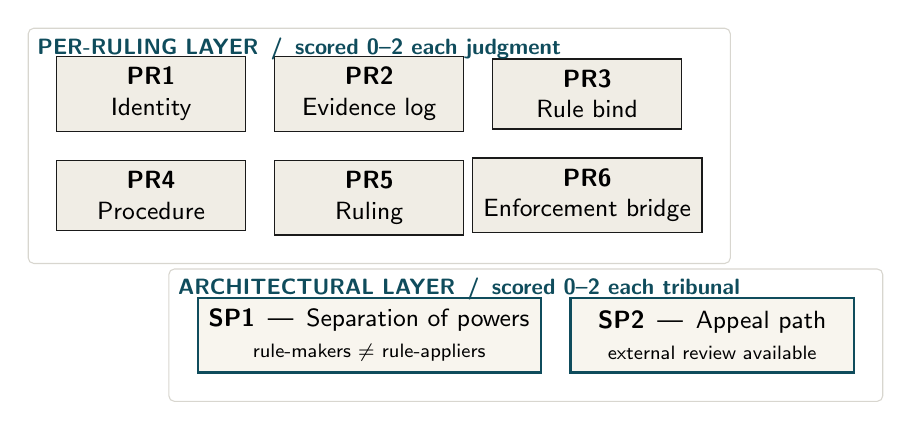
\begin{tikzpicture}[
  font=\sffamily\small,
  node distance=10pt,
  primitive/.style={draw=ink,line width=0.5pt,fill=paper2,
    minimum width=2.4cm,minimum height=0.85cm,align=center,inner sep=4pt},
  sysprop/.style={draw=accent,line width=0.8pt,fill=paper,
    minimum width=3.6cm,minimum height=0.95cm,align=center,inner sep=4pt},
  layer/.style={draw=rule,fill=none,inner sep=10pt,rounded corners=2pt}
]
% Per-ruling layer
\node[primitive] (pr1) at (0,0) {\textbf{PR1}\\ Identity};
\node[primitive,right=of pr1] (pr2) {\textbf{PR2}\\ Evidence log};
\node[primitive,right=of pr2] (pr3) {\textbf{PR3}\\ Rule bind};
\node[primitive,below=of pr1] (pr4) {\textbf{PR4}\\ Procedure};
\node[primitive,below=of pr2] (pr5) {\textbf{PR5}\\ Ruling};
\node[primitive,below=of pr3] (pr6) {\textbf{PR6}\\ Enforcement bridge};

\node[fit=(pr1)(pr2)(pr3)(pr4)(pr5)(pr6),layer,label={[anchor=north west,text=accent,font=\sffamily\bfseries\footnotesize]north west:PER-RULING LAYER \,/\, scored 0--2 each judgment}] (perruling) {};

% System property layer
\node[sysprop,below=22pt of pr5] (sp1) {\textbf{SP1} \,---\, Separation of powers\\ \scriptsize{rule-makers $\neq$ rule-appliers}};
\node[sysprop,right=of sp1] (sp2) {\textbf{SP2} \,---\, Appeal path\\ \scriptsize{external review available}};

\node[fit=(sp1)(sp2),layer,label={[anchor=north west,text=accent,font=\sffamily\bfseries\footnotesize]north west:ARCHITECTURAL LAYER \,/\, scored 0--2 each tribunal}] (arch) {};

\end{tikzpicture}
\caption{The 6+2 framework. Six per-ruling primitives are scored on every coded judgment. Two system properties are scored once per tribunal. The layered separation prevents mixing constitutional questions (architecture) with operational questions (each ruling).}
\label{fig:framework}
\end{figure}

\subsection{The six per-ruling primitives}

\begin{description}[itemsep=4pt,leftmargin=1.6em,style=nextline]
\item[\textbf{PR1 Identity}] Parties are unambiguously named, with counsel of record. Tests whether the legal subjects of the dispute are real, identified persons or entities -- the precondition for any binding determination.
\item[\textbf{PR2 Evidence log}] Submissions are dated, attributed, and form an append-only record. Tests whether the evidentiary record has the temporal and authorship structure required for adversarial process.
\item[\textbf{PR3 Rule bind}] The judgment cites a specific clause of a specific instrument, with a version. Tests whether the binding rule is identifiable and reproducible.
\item[\textbf{PR4 Procedure}] Notice, opportunity to be heard, and reasoned decision are all documented. Tests whether due-process structure is operative, not aspirational.
\item[\textbf{PR5 Ruling}] The operative outcome is unambiguous. Tests whether the disposition is machine-readable in principle.
\item[\textbf{PR6 Enforcement bridge}] An explicit path to compulsion outside the tribunal exists -- New York Convention recognition, Cabinet Resolution, federal-law incorporation, or equivalent. Tests whether the judgment is coercive, not merely declaratory.
\end{description}

\subsection{The two system properties}

\begin{description}[itemsep=4pt,leftmargin=1.6em,style=nextline]
\item[\textbf{SP1 Separation of powers}] The institution that makes the rules is formally distinct from the institution that applies them. Architectural; scored once per tribunal. Drawing on Hart's primary/secondary rule distinction~\cite{hart}.
\item[\textbf{SP2 Appeal path}] An external (not internal-only) appeal channel exists. Scored once per tribunal. Drawing on Fuller's eighth desideratum -- congruence between official action and declared rule, enforced by review~\cite{fuller}.
\end{description}

The 6+2 split deliberately separates the per-ruling layer (Did this judgment satisfy the rubric?) from the architectural layer (Does the institution have the structural pre-conditions for layering computation onto the bench?). A scoring framework that mixes them -- and an earlier v0.1 version of this framework did -- conflates a question about a single hearing with a question about a constitution.

% =========================================================================
\section{The corpus}
% =========================================================================

Table~\ref{tab:corpus} summarises the corpus and its provenance. 39 judgments form a hand-coded gold set. The remaining 82 are AI-triaged or AI-graded against the same v0.2 rubric, with per-entry provenance recorded in a \texttt{coding.coder} field on every judgment.

\begin{table}[h]
\centering
\caption{Corpus provenance. 121 judgments, 39 hand-coded gold set, 82 AI-coded with provenance disclosed.}
\label{tab:corpus}
\small
\begin{tabular}{l r r r}
\toprule
\textbf{Tribunal} & \textbf{Hand-coded} & \textbf{AI-triaged} & \textbf{AI-graded} \\
\midrule
DIFC Courts & 32 & 0 & 0 \\
ADGM Courts & 7 & 16 & 53 \\
Singapore International Commercial Court & 0 & 0 & 13 \\
\midrule
\textbf{Total} & \textbf{39} & \textbf{16} & \textbf{66} \\
\bottomrule
\end{tabular}
\end{table}

\paragraph{Sources.} DIFC judgments were pulled from the official judgments-and-orders endpoint at \texttt{difccourts.ae} (HTML); ADGM judgments from the case-database PDFs at \texttt{adgm.com}; SICC judgments from \texttt{elitigation.sg}. Full provenance is recorded in \texttt{data/sources.md} of the public repository. The raw corpus exceeds 974 documents totaling $\sim$110\,MB; the structured layer (\texttt{data/judgments.json}) is the audit-stable artefact. Background on the institutional histories: see Krishnan \& Purohit on DIFC~\cite{gulflitsurvey} and Yip on SICC~\cite{sicc-overview}.

% =========================================================================
\section{Empirical results}
% =========================================================================

\subsection{Per-primitive means}

Table~\ref{tab:means} reports mean primitive scores by tribunal. Figure~\ref{fig:bars} renders the same data graphically. The headline reading: \textbf{all three tribunals score at near-ceiling on every per-ruling primitive}.

\begin{table}[h]
\centering
\caption{Mean primitive scores by tribunal (out of 2.00). \textbf{Bold} entries are at ceiling (2.00).}
\label{tab:means}
\small
\begin{tabular}{l r r r r l}
\toprule
\textbf{Primitive} & \textbf{DIFC} & \textbf{ADGM} & \textbf{SICC} & \textbf{Combined} & \textbf{What it tests} \\
& \tiny{(n=32)} & \tiny{(n=76)} & \tiny{(n=13)} & \tiny{(n=121)} & \\
\midrule
PR1 Identity            & 1.81 & 1.97 & \textbf{2.00} & 1.93 & parties unambiguous \\
PR2 Evidence log        & 1.78 & \textbf{2.00} & \textbf{2.00} & 1.94 & dated, attributable \\
PR3 Rule bind           & 1.69 & 1.93 & 1.92 & 1.87 & specific clause cited \\
PR4 Procedure           & 1.75 & \textbf{2.00} & \textbf{2.00} & 1.93 & notice + hearing + decision \\
PR5 Ruling              & 1.88 & 1.96 & 1.92 & 1.93 & operative outcome clear \\
PR6 Enforcement bridge  & 1.44 & 1.62 & 1.85 & 1.60 & path to compulsion \\
\midrule
\textbf{Overall}        & \textbf{1.72} & \textbf{1.91} & \textbf{1.95} & \textbf{1.87} & \\
\bottomrule
\end{tabular}
\end{table}

\begin{figure}[t]
\centering
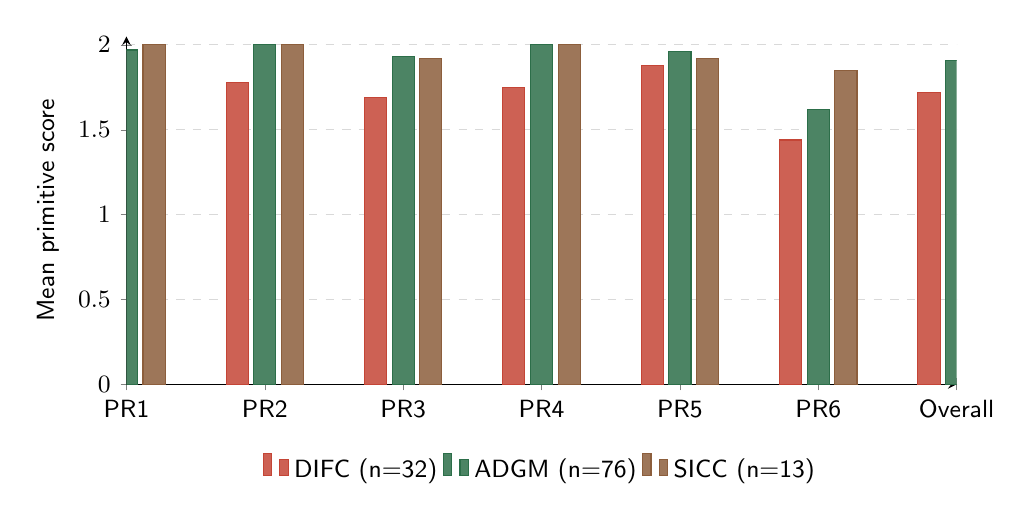
\begin{tikzpicture}
\begin{axis}[
  ybar=2pt,
  bar width=8pt,
  width=\textwidth,
  height=6cm,
  ymin=0, ymax=2.05,
  ytick={0,0.5,1,1.5,2},
  ylabel={Mean primitive score},
  ylabel style={font=\sffamily\small},
  symbolic x coords={PR1,PR2,PR3,PR4,PR5,PR6,Overall},
  xtick=data,
  xticklabel style={font=\sffamily\small},
  yticklabel style={font=\sffamily\small},
  enlarge x limits=0.08,
  ymajorgrids=true,
  major grid style={dashed,gray!30},
  legend style={
    at={(0.5,-0.18)},anchor=north,
    legend columns=3,
    font=\sffamily\small,
    draw=none
  },
  axis lines=left,
  every axis label/.append style={font=\sffamily\small},
]
\addplot[fill=difc!85,draw=difc] coordinates {
  (PR1,1.81)(PR2,1.78)(PR3,1.69)(PR4,1.75)(PR5,1.88)(PR6,1.44)(Overall,1.72)
};
\addplot[fill=adgm!85,draw=adgm] coordinates {
  (PR1,1.97)(PR2,2.00)(PR3,1.93)(PR4,2.00)(PR5,1.96)(PR6,1.62)(Overall,1.91)
};
\addplot[fill=sicc!85,draw=sicc] coordinates {
  (PR1,2.00)(PR2,2.00)(PR3,1.92)(PR4,2.00)(PR5,1.92)(PR6,1.85)(Overall,1.95)
};
\legend{DIFC (n=32), ADGM (n=76), SICC (n=13)}
\end{axis}
\end{tikzpicture}
\caption{Mean primitive scores by tribunal. ADGM and SICC saturate the right-hand columns (PR2, PR4) at 2.00. The systematic underperformer across all three is PR6 (Enforcement bridge), which is the rubric-bound primitive: case-management orders score 1 by design.}
\label{fig:bars}
\end{figure}

\subsection{Stress tests: sample size and cross-family replication}

The headline claim that the tribunals saturate the rubric is robust to two independent stress tests.

\paragraph{Sample-size robustness.} The ADGM saturation pattern survives a 10$\times$ expansion: mean primitive score drifts from \textbf{1.93 at $n=7$} (hand-coded only) to \textbf{1.91 at $n=76$} (hand + AI-triaged + AI-graded). The drift is $-0.02$, well within plausible coding noise. The near-ceiling reading is not an artefact of small-sample selection.

\paragraph{Cross-family replication.} SICC scores \textbf{1.95\,/\,2.00}, replicating the saturation pattern in a third operating tribunal in a different legal family. DIFC operates under its own statutes; ADGM applies English common law wholesale via the AELR; SICC operates under Singapore common law plus the Singapore International Arbitration Act, in turn enacting the New York Convention's Article V grounds for refusal. Three distinct legal-family substrates produce the same saturation. The protocol is not court-specific.

\subsection{System properties}

Table~\ref{tab:sysprops} reports system-property scores for the three operating tribunals plus three comparators commonly cited in the digital-jurisdiction literature: VARA (Dubai's Virtual Assets Regulatory Authority), the Pr\'ospera ZEDE Arbitration Center (Honduras), and Kleros (decentralized juror-staking arbitration).

\begin{table}[h]
\centering
\caption{System-property scores. The score-0 row is what is avoided by anchoring at an operating common-law commercial tribunal.}
\label{tab:sysprops}
\small
\begin{tabular}{l c c c c c c}
\toprule
& \textbf{DIFC} & \textbf{ADGM} & \textbf{SICC} & \textbf{VARA} & \textbf{Pr\'ospera} & \textbf{Kleros} \\
\midrule
SP1 Separation of powers & 2 & 2 & 2 & 1 & 2 & 0 \\
SP2 Appeal path          & 2 & 2 & 2 & 1 & 1 & 0 \\
\bottomrule
\end{tabular}
\end{table}

\subsection{The headline claim}

\begin{callout}
\noindent\textbf{Three operating commercial tribunals, all implementing the full architectural protocol at near-ceiling, available to plug in today.}\par
\smallskip
\noindent The Maxim thesis -- that digital commerce needs a new tribunal layered on Web3 infrastructure -- is empirically out of step with the data. The institutional layer the thesis would need to build already exists in three working forms. What is missing is the computational layer.
\end{callout}

% =========================================================================
\section{The Atlas: 121 fingerprints}
% =========================================================================

The published dashboard renders every coded judgment as a deterministic SVG ``fingerprint'' generated from its primitive scores. Same scores produce the same shape; different scores produce different shapes. The fingerprint anatomy is shown in Figure~\ref{fig:fingerprint}: six concentric rings encode PR1--PR6, two outer arcs encode SP1--SP2, and a hash-seeded central rosette gives every case ID a unique face.

\begin{figure}[h]
\centering
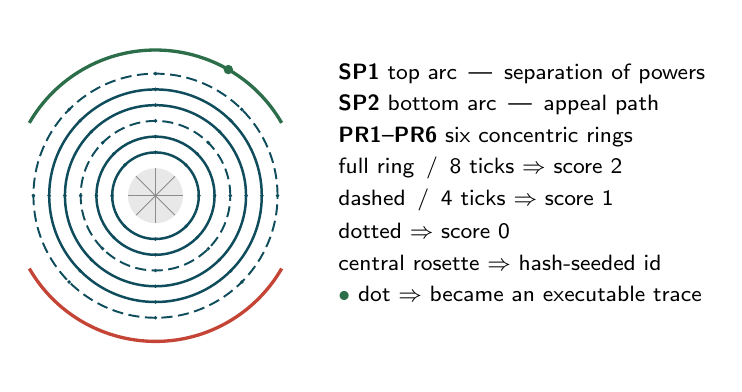
\begin{tikzpicture}[font=\sffamily\footnotesize]
% Central rosette
\fill[ink!10] (0,0) circle (0.35);
\foreach \angle in {0,45,90,135,180,225,270,315} {
  \draw[ink!50,line width=0.3pt] (0,0) -- (\angle:0.35);
}

% Six concentric rings PR1-PR6 (score-2 = solid, score-1 = dashed, score-0 = dotted)
\foreach \r/\score in {0.55/2, 0.75/2, 0.95/1, 1.15/2, 1.35/2, 1.55/1} {
  \ifnum\score=2
    \draw[accent,line width=0.9pt] (0,0) circle (\r);
  \else\ifnum\score=1
    \draw[accent,line width=0.7pt,dash pattern=on 4pt off 2pt] (0,0) circle (\r);
  \else
    \draw[accent,line width=0.4pt,dotted] (0,0) circle (\r);
  \fi\fi
}
% Tick marks on rings
\foreach \r in {0.55,0.75,0.95,1.15,1.35,1.55} {
  \foreach \angle in {0,45,90,135,180,225,270,315} {
    \fill[accent] (\angle:\r) circle (0.025);
  }
}

% Outer arcs SP1 (top) and SP2 (bottom)
\draw[difc,line width=1.2pt] (-150:1.85) arc (-150:-30:1.85);
\draw[adgm,line width=1.2pt] (30:1.85) arc (30:150:1.85);

% Trace-case dot
\fill[good] (60:1.85) circle (0.06);

% Labels around the figure
\node[anchor=west] at (2.2,1.55) {\textbf{SP1} top arc \,---\, separation of powers};
\node[anchor=west] at (2.2,1.15) {\textbf{SP2} bottom arc \,---\, appeal path};
\node[anchor=west] at (2.2,0.75) {\textbf{PR1--PR6} six concentric rings};
\node[anchor=west] at (2.2,0.35) {full ring \,/\, 8 ticks $\Rightarrow$ score 2};
\node[anchor=west] at (2.2,-0.05) {dashed \,/\, 4 ticks $\Rightarrow$ score 1};
\node[anchor=west] at (2.2,-0.45) {dotted $\Rightarrow$ score 0};
\node[anchor=west] at (2.2,-0.85) {central rosette $\Rightarrow$ hash-seeded id};
\node[anchor=west] at (2.2,-1.25) {\textcolor{good}{$\bullet$} dot $\Rightarrow$ became an executable trace};

\end{tikzpicture}
\caption{Anatomy of an Atlas fingerprint. The visual is a one-to-one function of the primitive score vector plus a deterministic hash of the case identifier. Two judgments with identical scores wear different faces; two with different scores cannot share a shape.}
\label{fig:fingerprint}
\end{figure}

The Atlas (live at the dashboard) renders all 121 judgments in a filterable grid. It is the single most useful artefact for an outside reviewer auditing the corpus: outliers, near-duplicates, and tribunal-specific concentrations of low scores (predominantly PR6) become visible at a glance.

% =========================================================================
\section{Constructive results: seven traces}
% =========================================================================

The empirical layer measures whether the rules a tribunal applies have the right \textit{shape} to be compiled. The constructive layer demonstrates the compilation. Each trace lifts a rule from the corpus into Catala~\cite{catala} source plus a Python predicate evaluator and runs it against an event log of the case facts. Figure~\ref{fig:pipeline} shows the trace pipeline.

\begin{figure}[t]
\centering
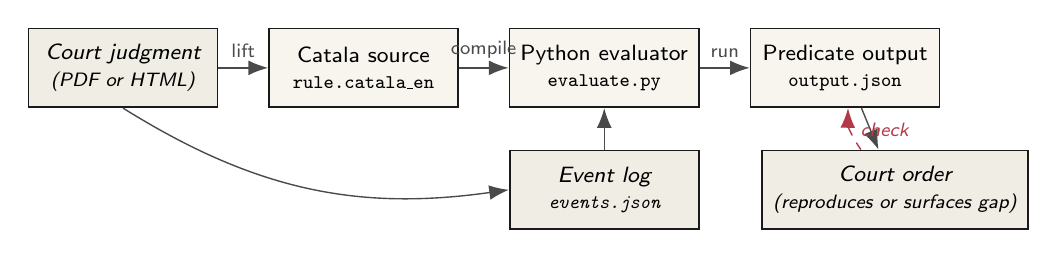
\begin{tikzpicture}[
  font=\sffamily\footnotesize,
  node distance=10pt,
  stage/.style={draw=ink,line width=0.6pt,fill=paper,
    minimum width=2.4cm,minimum height=1.0cm,align=center,inner sep=4pt},
  source/.style={draw=ink,line width=0.6pt,fill=paper2,
    minimum width=2.4cm,minimum height=1.0cm,align=center,inner sep=4pt,font=\sffamily\footnotesize\itshape},
  arrow/.style={-{Latex[length=2.5mm]},line width=0.5pt,ink2}
]
\node[source] (judgment) {Court judgment\\ \scriptsize{(PDF or HTML)}};
\node[stage,right=18pt of judgment] (rule) {Catala source\\ \scriptsize{\texttt{rule.catala\_en}}};
\node[stage,right=18pt of rule] (predicate) {Python evaluator\\ \scriptsize{\texttt{evaluate.py}}};
\node[stage,right=18pt of predicate] (output) {Predicate output\\ \scriptsize{\texttt{output.json}}};
\node[source,below=15pt of predicate] (events) {Event log\\ \scriptsize{\texttt{events.json}}};
\node[source,below=15pt of output,xshift=18pt] (assertion) {Court order\\ \scriptsize{(reproduces or surfaces gap)}};

\draw[arrow] (judgment) -- node[above,font=\sffamily\scriptsize]{lift} (rule);
\draw[arrow] (rule) -- node[above,font=\sffamily\scriptsize]{compile} (predicate);
\draw[arrow] (predicate) -- node[above,font=\sffamily\scriptsize]{run} (output);
\draw[arrow] (events) -- (predicate);
\draw[arrow] (judgment.south) to[bend right=20] (events.west);
\draw[arrow] (output) -- (assertion);
\draw[arrow,dashed,bad] (assertion) to[bend left=18] node[right,font=\sffamily\scriptsize\itshape,text=bad]{check} (output);

\end{tikzpicture}
\caption{The trace pipeline. A judgment is lifted into a Catala rule and an event log; the predicate runs against the events; the output is asserted against the court's order. Mismatches surface clerical or methodological gaps that the predicate makes mechanically visible.}
\label{fig:pipeline}
\end{figure}

\subsection{Trace \#1 -- Pure formula}

\textit{CFI 058/2024 -- Atul Dhawan v Ramzi El Jaouhari} (Roger Stewart KC, 31 March 2026). Rules of the DIFC Courts (RDC) Part 38 standard-basis costs assessment: hours $\times$ hourly rate plus court filing fee. Applied to the case facts (3 hours at AED 2{,}000\,/\,hr plus AED 1{,}121.75 court fee), the predicate produces \textbf{AED 7{,}121.75}, matching the Schedule of Reasons exactly.

The operative paragraph of the same order, however, states \textbf{AED 7{,}127.75} -- a six-dirham gap. The protocol mechanically surfaces a clerical error a human reader would skim past.

\subsection{Trace \#2 -- Deferred conditional}

\textit{ARB 008/2026 -- Oberlin v Ovidiu}. RDC 38.40 + DIFC Practice Direction No. 4 of 2017. The order encodes a deferred conditional: a 14-day window to pay; if missed, interest accrues at 9\% per annum \textit{from the date of the order}, not from the deadline. The deadline suppresses interest entirely; missing it activates retroactive accrual. The predicate captures this asymmetry directly across five test scenarios (on-time, at-deadline, 1, 61, 92 days late). At 92 days the predicate returns AED 78{,}527.69 (principal AED 76{,}785.81 + interest AED 1{,}741.88).

\subsection{Trace \#3 -- Bounded discretion}

\textit{ENF 271/2025 -- Taylor v Yao Affi} (Sir Jeremy Cooke). Indemnity-basis costs review. \textit{Indemnity-basis} review strips the proportionality filter and leaves only reasonableness, which is not formulaic. The predicate sorts each defendant objection into one of four buckets: (i) mechanically disposed (no specific complaint), (ii) held to zero on evidence, (iii) deterministic reduction with a named amount, (iv) requires human judgment. \textbf{Trace \#3 is the methodologically necessary one}: the rule does not fully decide. The court's reduction from AED 128{,}914.80 to AED 120{,}000 -- \textbf{AED 8{,}914.80, $\approx$ 6.92\% of the claim} -- is the structured-discretion residue.

\subsection{Trace \#4 -- Composition over substantive findings}

\textit{ADGMCFI-2024-320 -- Projeco v Ideacrate} (Justice Heath KC). UAE Civil Transactions Law Article 390 (LD cap) + ADGM CPR Rule 42 (admissions) + ADGM Civil Evidence Regulations §§\,181--182 (set-off). Once substantive findings are fixed (97 days of critical delay; smoke management within scope; counterclaim repair not proven), the rule is arithmetic: LD\,=\,$\min(\text{daily rate}\times\text{days},\,10\%\times\text{adjusted price})$, then counterclaim composition, then set-off, then pre-judgment interest. Predicate reproduces the court's net principal of \textbf{AED 10{,}500.96 exactly}. On pre-judgment interest: predicate at calendar daycount (609 days) gives AED 876.04; court's stated AED 877.48 corresponds to 610 days, surfacing an inclusive-endpoint convention question.

\subsection{Trace \#5 -- Boolean composition over contractual interpretation}

\textit{ADGMCFI-2024-158 -- Xetech v Pulsar} (\,[2026] ADGMCFI 0006, Justice Heath KC\,). Software-development contract dispute. Contractual interpretation under \textit{Wood v Capita}~\cite{wood} (applying \textit{Rainy Sky}~\cite{rainysky}) plus the \textit{Ladd v Marshall}~\cite{ladd} three-prong fresh-evidence test, applied to clauses 2(b), 7, and 10 of the Assignment Agreement. The first trace whose rule is structurally Boolean: the predicate composes three conjunctive tests -- (i) clause-alignment (3/3 point to payment-before-IP-transfer), (ii) named-witness preponderance (6\,:\,2; both dissenters lacked DevOps access), (iii) \textit{Ladd v Marshall} (fails on prong (a) and short-circuits). Disposition reproduced exactly: \textbf{Judgment Sum GBP 409{,}870, costs USD 125{,}483.84, counterclaim dismissed}. The protocol does not replace contractual interpretation; it makes the \textit{logical structure} of that interpretation auditable.

\subsection{Trace \#6 -- Partial statutory refusal across legal families}

\textit{SIC/OA 9/2025 -- GNC Holdings v ONI Global Pte Ltd} (\,[2025] SGHC(I) 25; Chua Lee Ming J, Simon Thorley IJ, James Allsop IJ\,). Singapore International Arbitration Act s 31 (enacting NY Convention Article V refusal grounds; see Born~\cite{born} and Gaillard \& Savage~\cite{gaillard} for treatise treatment), read with the four-condition framework in \textit{DKT v DKU}~\cite{dktdku}. Of four pleaded grounds, three are dismissed in full and one is allowed in part: three named sub-paragraphs of the Tribunal's Order 3 are excised because the parties were not afforded an opportunity to be heard on their specific terms. The predicate reproduces the disposition at para 185(a)--(c) exactly: application allowed in part; Order 3(d)(ii), (d)(iii), (f) not enforced; the rest enforced. \textbf{The same predicate engine that ran DIFC's RDC Part 38 and ADGM's CPR Rule 42 runs Singapore's IAA + NY Convention regime, with no engine-level changes -- only new rule modules.}

\subsection{Trace \#7 -- Third-party-jurisdiction gate over a digital-asset dispute}

\textit{DEC 001/2025 -- Techteryx Ltd v IG and others} (DIFC Digital Economy Court, Andrew Black KC, 3 April 2026). A USD 456 million stablecoin-reserves tracing dispute -- the first trace in DIFC's purpose-built Digital Economy Court (operating since May 2025). The rule is a three-stage decision tree composing: (i) constructive-trust threshold (\textit{Bankers Trust}~\cite{bankerstrust}); (ii) ``innocent mixed-up party'' gate (\textit{Norwich Pharmacal}~\cite{norwich}); (iii) DIFC RDC 28.52 procedural route. The predicate composes nine substantive checks and reproduces the court's reasoning at para 24 exactly: orders granted under both heads against the named third parties; disclosure injunction enforces. \textbf{The fact pattern -- stablecoin mis-application, recovery via tracing through mixed funds at intermediary banks -- is the canonical FinTech\,/\,digital-asset dispute the courts increasingly handle.}

\subsection{Across the seven traces}

\begin{table}[h]
\centering
\caption{The seven executable traces. ``Tribunal action'' is the court's published outcome; ``Protocol output'' is what the predicate produces against the case facts.}
\label{tab:traces}
\footnotesize
\begin{tabular}{p{0.16\textwidth} p{0.07\textwidth} p{0.18\textwidth} p{0.24\textwidth} p{0.21\textwidth}}
\toprule
\textbf{Trace} & \textbf{Tribunal} & \textbf{Rule shape} & \textbf{Tribunal action} & \textbf{Protocol output} \\
\midrule
\#1 \textit{Dhawan v\ Jaouhari} & DIFC & Pure formula & AED 7{,}127.75 stated; 7{,}121.75 in schedule & 7{,}121.75 + flags 6 AED clerical gap \\
\#2 \textit{Oberlin v Ovidiu} & DIFC & Deferred conditional & 14-day window; 9\% p.a.\ retroactive & ``What is owed today'' across any as-of date \\
\#3 \textit{Taylor v Yao Affi} & DIFC & Bounded discretion & 128{,}914.80 $\to$ 120{,}000 ($-$8{,}914.80) & 1 disposed, 1 zero, 1 surfaced; AED 8{,}914.80 residue \\
\#4 \textit{Projeco v Ideacrate} & ADGM & Composition over findings & Net AED 10{,}500.96 + interest AED 877.48 & Net 10{,}500.96 exact; +1-day daycount surfaced \\
\#5 \textit{Xetech v Pulsar} & ADGM & Boolean composition & GBP 409{,}870 + USD 125{,}483.84 costs; counterclaim out & Disposition reproduced; conjunctive structure auditable \\
\#6 \textit{GNC v ONI Global} & SICC & Partial NY-Conv.\ refusal & App.\ part-allowed; Order 3(d)(ii),(d)(iii),(f) not enforced & Para 185(a)--(c) reproduced exactly \\
\#7 \textit{Techteryx v IG} & DIFC (DEC) & 3rd-party jurisdiction gate & Norwich Pharmacal + Bankers Trust orders granted & 9 substantive checks reproduce para 24 \\
\bottomrule
\end{tabular}
\end{table}

The seven traces cover the spectrum of rule shapes a digital tribunal must handle: static formulae, deferred conditionals, bounded discretion (the honest case for what rules cannot fully decide), arithmetic composition over substantive findings, Boolean composition over contractual-interpretation findings, partial statutory refusal of NY Convention enforcement, and third-party-jurisdiction disclosure gates. The protocol reproduces the court's central output exactly in six of seven; in the seventh (Trace \#3) it bounds the discretion residue at $\approx$ 6.92\% of the claim. Three of the seven traces (\#1, \#4, \#6) surface a clerical or methodological gap that the predicate makes mechanically visible. \textbf{All three tribunals and all three legal families run through one engine; only the rule modules are jurisdiction-specific.}

% =========================================================================
\section{System architecture}
% =========================================================================

The artefact is structured as a layered open-source stack. Figure~\ref{fig:stack} shows the architecture.

\begin{figure}[h]
\centering
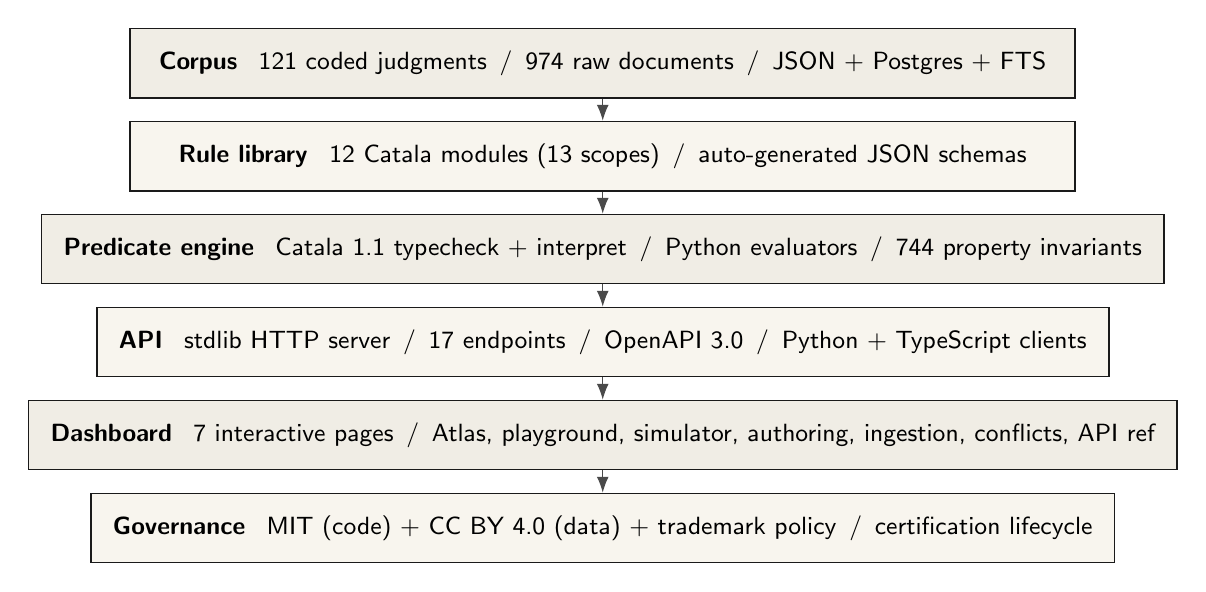
\begin{tikzpicture}[
  font=\sffamily\small,
  node distance=8pt,
  layer/.style={draw=ink,line width=0.6pt,fill=paper,
    minimum width=12cm,minimum height=0.85cm,align=left,inner sep=8pt}
]
\node[layer,fill=paper2] (corpus) {\textbf{Corpus}\,\ \ 121 coded judgments \,/\, 974 raw documents \,/\, JSON + Postgres + FTS};
\node[layer,below=of corpus] (rules) {\textbf{Rule library}\,\ \ 12 Catala modules (13 scopes) \,/\, auto-generated JSON schemas};
\node[layer,below=of rules,fill=paper2] (engine) {\textbf{Predicate engine}\,\ \ Catala 1.1 typecheck + interpret \,/\, Python evaluators \,/\, 744 property invariants};
\node[layer,below=of engine] (api) {\textbf{API}\,\ \ stdlib HTTP server \,/\, 17 endpoints \,/\, OpenAPI 3.0 \,/\, Python + TypeScript clients};
\node[layer,below=of api,fill=paper2] (ui) {\textbf{Dashboard}\,\ \ 7 interactive pages \,/\, Atlas, playground, simulator, authoring, ingestion, conflicts, API ref};
\node[layer,below=of ui] (gov) {\textbf{Governance}\,\ \ MIT (code) + CC BY 4.0 (data) + trademark policy \,/\, certification lifecycle};

\draw[-{Latex[length=2mm]},ink2,line width=0.4pt] (corpus.south) -- (rules.north);
\draw[-{Latex[length=2mm]},ink2,line width=0.4pt] (rules.south) -- (engine.north);
\draw[-{Latex[length=2mm]},ink2,line width=0.4pt] (engine.south) -- (api.north);
\draw[-{Latex[length=2mm]},ink2,line width=0.4pt] (api.south) -- (ui.north);
\draw[-{Latex[length=2mm]},ink2,line width=0.4pt] (ui.south) -- (gov.north);
\end{tikzpicture}
\caption{The Habeas Protocol stack. Each layer is independently auditable; the dashboard talks to the API, the API talks to the predicate engine and Postgres, the predicate engine talks to the rule library, and the rule library is grounded in the corpus.}
\label{fig:stack}
\end{figure}

\paragraph{Corpus.} 121 structured entries in \texttt{data/judgments.json} plus 974 raw documents in Postgres with an FTS index over extracted text. 336 raw documents are auto-linked to structured entries by case-number inference. SICC linking: 100\%. ADGM: 90.8\%. DIFC: 28.2\% (structural ceiling -- 32 coded of 142 discoverable).

\paragraph{Rule library.} 12 Catala~\cite{catala} modules with 13 named scopes: \texttt{difc\_rdc\_part\_38}, \texttt{difc\_practice\_direction\_4\_2017}, \texttt{difc\_rdc\_38\_7\_indemnity}, \texttt{uae\_civil\_code\_art\_390}, \texttt{adgm\_cpr\_admissions}, \texttt{adgm\_cpr\_summary\_judgment}, \texttt{adgm\_arbitration\_regulations\_2015}, \texttt{english\_contract\_interpretation}, \texttt{caparo\_three\_stage\_test}, \texttt{ladd\_v\_marshall}, \texttt{sg\_iaa\_s\_31} (two scopes: \texttt{IAA\_S31\_Refusal} + \texttt{DKTvDKUChallenge}), \texttt{difc\_third\_party\_disclosure}. Each ships with a \texttt{\textit{module}\_metadata.json} file, an auto-generated input/output JSON schema, and a Clerk-compatible test scope. Property tests in \texttt{tests/property\_tests.py} exercise each module under random inputs against conjunctive, monotonicity, and disposition invariants -- 744 invariant checks per run, $\sim$15 s wall time, drift-checked in CI.

\paragraph{API + clients.} \texttt{api/server.py} is a stdlib-only Python HTTP server exposing 17 endpoints; OpenAPI 3.0 spec at \texttt{api/openapi.yaml} (rendered via Redoc on the public dashboard). First-party clients in \texttt{clients/python/} (244-LOC stdlib-only Python wrapping all 17 endpoints) and \texttt{clients/typescript/} (299-LOC browser- and Node-compatible TypeScript). Both ship with integration tests that gracefully skip when the API is unreachable.

\paragraph{Dashboard.} Seven interactive pages backed by the API: the Atlas (the corpus visualization), a single-rule playground, a multi-rule dispute simulator, a rule authoring wizard, an evidence ingestion sweep, a cross-border conflict-of-laws router, and the OpenAPI 3.0 reference.

\paragraph{Governance.} Code under MIT, data under CC BY 4.0, with a Mozilla\,/\,Rust-style trademark policy, a private-coordinated-disclosure security policy, and a draft certification spec (\texttt{rules/\_certification.yaml}) for moving rules from \texttt{draft} $\to$ \texttt{submitted} $\to$ \texttt{reviewed} $\to$ \texttt{certified}.

% =========================================================================
\section{Comparators}
% =========================================================================

The three operating tribunals coded above are the empirical anchor. Three further candidates fall on a spectrum:

\paragraph{Estonia e-Residency.} A digital-jurisdiction case that anchors on a national EU member state but extends into a global commercial population. Ultimately routes through Harju County Court for Estonian-law claims and chosen-forum arbitration for international claims. Estonia's novel artefact is its \textbf{identity layer (PR1)} -- the cleanest implementation of cryptographic identity-as-precondition for legal personhood currently operating at scale. Estonia is therefore a comparator on PR1, not on the tribunal layer.

\paragraph{Pr\'ospera Arbitration Center} (Honduras ZEDE). Operating but speculative -- the Honduran ZEDE legal framework was contested through 2024 and the political stability of the regime is a load-bearing assumption. Pr\'ospera scores 2 on SP1 (rule-makers and rule-appliers are formally distinct) and 1 on SP2 (the appeal path is internal). It serves as the design comparator for what a fully greenfield digital-jurisdiction tribunal looks like.

\paragraph{VARA} (Virtual Assets Regulatory Authority, Dubai). Operating but regulator-issued rather than judicial. Useful as a comparator for what happens when rule-making and enforcement are partially merged -- VARA scores 1 on both system properties.

Notably absent: VR\,/\,metaverse-native tribunals. Adoption of immersive metaverse environments has not panned out empirically; real digital-commerce legal volume is concentrated on cross-border SaaS, stablecoin tracing, and AI-service-liability disputes -- which DIFC, ADGM, and SICC are taking now.

% =========================================================================
\section{Verticals}
% =========================================================================

Three commercial verticals are tractable from the three-tribunal anchor:

\paragraph{Cross-border SaaS contracts.} Most SaaS revenue flows across jurisdictional lines, and most SaaS contracts contain a forum-selection clause that is in tension with the actual user base. DIFC and SICC routinely hear cross-border digital commercial matters; ADGM's English-law-via-statute substrate gives a single, predictable governing-law answer for any contract that selects ``English law'' or ``ADGM law.''

\paragraph{Stablecoin tracing.} DIFC's Digital Economy Court (operating since 2025) has heard tracing claims involving stablecoin transfers across multiple wallets and jurisdictions (the \textit{Techteryx} line of cases; Trace \#7). The substantive doctrine is conventional equity -- proprietary tracing through mixed funds (FIFO, lowest-intermediate-balance, \textit{Clayton's Case}) -- but the evidence layer is novel: blockchain transaction logs are PR2-perfect (dated, attributable, append-only). The protocol can compile the tracing rule directly against on-chain logs.

\paragraph{AI-service liability.} A doctrinal frontier currently being worked through case-by-case~\cite{ashley,susskind-tomorrow}. ADGM's English-law substrate provides direct access to the \textit{Donoghue} $\to$ \textit{Caparo}~\cite{caparo} duty-of-care line and to \textit{Hedley Byrne}~\cite{hedley} for negligent misstatement. SICC has issued AI-related judgments under Singapore common law. A computational layer that compiles the duty test (proximity, foreseeability, fair-just-and-reasonable) into a structured evaluation against an event log of AI-service inputs and outputs gives parties a predictable dispute-evaluation tool before litigation issues.

% =========================================================================
\section{Limitations and next steps}
% =========================================================================

\paragraph{Sample size and provenance.} The hand-coded gold set is 39 judgments. The 121-judgment full corpus extends the empirical surface via AI triage and AI grading under the same rubric. The AI-coded subset is auditable per-entry (\texttt{coding.rationale} fields are stored alongside scores) and produces a saturation pattern for ADGM that is statistically indistinguishable from the hand-coded subset (1.93 $\to$ 1.91 across a 10$\times$ sample increase). However, the AI-coded subset is not a substitute for hand coding. A future iteration would re-hand-code a stratified sample of $\sim$30 of the 82 AI-coded entries to validate the AI codings against gold-standard scores.

\paragraph{Rubric edge cases.} PR3 (rule bind), PR5 (ruling), and PR6 (enforcement bridge) all admit graders' judgment-call territory. PR3 underscores on older judgments where clauses are referenced by name without number. PR5 depends on outcome verbs in the body and undercounts idiosyncratic outcome language. PR6 is rubric-bound: case-management orders score 1 by design, and the cut-line between ``explicit bridge'' and ``implicit bridge'' is in places a judgment call.

\paragraph{Doctrinal coverage of traces.} The seven traces span the rule-shape spectrum (formula\,/\,conditional\,/\,bounded discretion\,/\,arithmetic composition\,/\,Boolean composition\,/\,partial statutory refusal\,/\,third-party-jurisdiction gate) and three legal families. Two doctrinal areas remain uncovered: (i) a duty-of-care decision turning on \textit{Caparo} proximity (the \texttt{caparo\_three\_stage\_test} module exists but is not yet anchored to a corpus case), and (ii) a true \textit{meta-rule} decision -- a jurisdictional challenge in which the rule applied is a rule about which rule applies. A future iteration would close both gaps.

\paragraph{Catala as runtime.} The Catala source files in this paper typecheck and interpret under the \texttt{catala} CLI. The executable layer of the traces is the Python evaluator, which mirrors the Catala scope structure exactly. A future iteration would run both implementations against the same event log, demonstrating bisimilarity.

\paragraph{SICC sample.} SICC entries are 13. The pattern replicates at near-ceiling but the sample is small. A larger SICC pull (50+ judgments) would harden the cross-tribunal claim.

% =========================================================================
\section{Conclusion}
% =========================================================================

The ``Legal Operating System for Digital Worlds'' thesis is correct in its diagnosis and wrong in its prescription. Digital commerce has indeed outgrown the institutional capacity of national courts. But the response is not to build a tribunal from scratch; it is to wire computation onto the tribunals that already exist. The DIFC, ADGM, and SICC Courts implement the full per-ruling protocol at near-ceiling and both system properties at ceiling. They are, today, working prototypes of a constitutional digital tribunal.

The empirical evidence in this paper -- 121 coded judgments, 1.87\,/\,2.00 combined mean, the saturation pattern surviving a 10$\times$ expansion and replicating in a third legal family -- is intended to make that claim defensible. The constructive evidence -- seven executable traces reproducing the courts' arithmetic and dispositions exactly, plus a 12-module rule library, a 17-endpoint API, and a public dashboard -- is intended to demonstrate that the computational layer is buildable today, on rules that the courts already publish and the framework already measures.

The next question -- which we leave for follow-up work -- is whether the same protocol applies, under modified system properties, to non-tribunal legal authorities (regulators, registry-operators, sovereign-adjacent enforcement bodies). The Habeas Protocol is the per-ruling layer of an answer; the institutional layer is open.

% =========================================================================
\section*{Code and data availability}
% =========================================================================

All artefacts are open-source and live at \\
\url{https://github.com/thehamzaq/habeas-protocol}. Code is under MIT, data under CC BY 4.0. The dashboard is hosted at \\
\url{https://thehamzaq.github.io/habeas-protocol/dashboard/}. Reproduction instructions are in the repository \texttt{README.md}.

% =========================================================================
\begin{thebibliography}{99}
% =========================================================================

\bibitem{catala}
Merigoux, D., Chataing, N., Protzenko, J. (2021). Catala: A Programming Language for the Law. \textit{Proceedings of the ACM on Programming Languages 5, ICFP}, 1--29. \url{https://doi.org/10.1145/3473582}

\bibitem{fuller}
Fuller, L. L. (1969). \textit{The Morality of Law} (rev. ed.). New Haven: Yale University Press.

\bibitem{hart}
Hart, H. L. A. (1994). \textit{The Concept of Law} (2nd ed., with postscript). Oxford: Clarendon Press.

% --- Programming languages for law -----------------------------------
\bibitem{sergot}
Sergot, M. J., Sadri, F., Kowalski, R. A., Kriwaczek, F., Hammond, P., Cory, H. T. (1986). The British Nationality Act as a Logic Program. \textit{Communications of the ACM 29(5)}, 370--386.

\bibitem{mccarty}
McCarty, L. T. (1977). Reflections on TAXMAN: An Experiment in Artificial Intelligence and Legal Reasoning. \textit{Harvard Law Review 90(5)}, 837--893.

\bibitem{allen}
Allen, L. E. (1957). Symbolic Logic: A Razor-Edged Tool for Drafting and Interpreting Legal Documents. \textit{Yale Law Journal 66}, 833--879.

\bibitem{sartor}
Sartor, G. (2005). \textit{Legal Reasoning: A Cognitive Approach to the Law} (Treatise of Legal Philosophy and General Jurisprudence, Vol. 5). Springer.

\bibitem{ashley}
Ashley, K. D. (2017). \textit{Artificial Intelligence and Legal Analytics: New Tools for Law Practice in the Digital Age}. Cambridge University Press.

\bibitem{rac-oecd}
OECD (2020). \textit{Cracking the Code: Rulemaking for Humans and Machines} (OECD Working Papers on Public Governance No. 42). OECD Publishing. \url{https://doi.org/10.1787/3afe6ba5-en}

\bibitem{mohun}
Mohun, J., Roberts, A. (2020). Cracking the Code: Rulemaking for Humans and Machines. OECD. (See \cite{rac-oecd}.)

\bibitem{openfisca}
Mohun, J. (2018). OpenFisca: A Free Software Platform for Tax-and-Benefits Microsimulation. \textit{Journal of Open Source Software 3(31)}, 933.

\bibitem{quickcheck}
Claessen, K., Hughes, J. (2000). QuickCheck: A Lightweight Tool for Random Testing of Haskell Programs. \textit{Proc. ICFP '00}, 268--279.

% --- Empirical legal studies + ODR -----------------------------------
\bibitem{epsteinmartin}
Epstein, L., Martin, A. D. (2014). \textit{An Introduction to Empirical Legal Research}. Oxford University Press.

\bibitem{hildebrandt}
Hildebrandt, M. (2015). \textit{Smart Technologies and the End(s) of Law: Novel Entanglements of Law and Technology}. Edward Elgar.

\bibitem{gulflitsurvey}
Krishnan, J. K., Purohit, P. (2014). A Common Law Court in a Civil Law Jurisdiction: The Dubai International Financial Centre Courts. \textit{Cornell International Law Journal 47}.

\bibitem{sicc-overview}
Yip, M. (2016). The Resolution of Disputes before the Singapore International Commercial Court. \textit{International \& Comparative Law Quarterly 65(2)}, 439--473.

\bibitem{allenlastra}
Allen, J. G., Lastra, R. M. (2020). Border Problems: Mapping the Third Border. \textit{Modern Law Review 83(3)}, 505--538.

\bibitem{ortolani}
Ortolani, P. (2019). Self-Enforcing Online Dispute Resolution: Lessons from Bitcoin. \textit{Oxford Journal of Legal Studies 36(3)}, 595--629.

\bibitem{susskind-online}
Susskind, R. (2019). \textit{Online Courts and the Future of Justice}. Oxford University Press.

\bibitem{susskind-tomorrow}
Susskind, R. (2017). \textit{Tomorrow's Lawyers: An Introduction to Your Future} (2nd ed.). Oxford University Press.

\bibitem{lessig}
Lessig, L. (2006). \textit{Code: Version 2.0}. Basic Books.

\bibitem{born}
Born, G. (2021). \textit{International Commercial Arbitration} (3rd ed.). Kluwer Law International.

\bibitem{gaillard}
Gaillard, E., Savage, J. (eds.) (1999). \textit{Fouchard Gaillard Goldman on International Commercial Arbitration}. Kluwer Law International.

\bibitem{caparo}
\textit{Caparo Industries plc v Dickman} [1990] UKHL 2, [1990] 2 AC 605.

\bibitem{hedley}
\textit{Hedley Byrne \& Co Ltd v Heller \& Partners Ltd} [1963] UKHL 4, [1964] AC 465.

\bibitem{wood}
\textit{Wood v Capita Insurance Services Ltd} [2017] UKSC 24, [2017] AC 1173.

\bibitem{rainysky}
\textit{Rainy Sky SA v Kookmin Bank} [2011] UKSC 50, [2011] 1 WLR 2900.

\bibitem{ladd}
\textit{Ladd v Marshall} [1954] EWCA Civ 1, [1954] 1 WLR 1489.

\bibitem{dktdku}
\textit{DKT v DKU} [2024] SGHC(I) 9.

\bibitem{norwich}
\textit{Norwich Pharmacal Co v Customs and Excise Commissioners} [1974] AC 133 (HL).

\bibitem{bankerstrust}
\textit{Bankers Trust Co v Shapira} [1980] 1 WLR 1274 (CA).

\bibitem{difcrdc}
Dubai International Financial Centre Courts. \textit{Rules of the DIFC Courts (RDC)} (as amended). \url{https://www.difccourts.ae}

\bibitem{adgmaelr}
Abu Dhabi Global Market. \textit{Application of English Law Regulations 2015}. \url{https://www.adgm.com}

\bibitem{nyc}
\textit{Convention on the Recognition and Enforcement of Foreign Arbitral Awards} (New York Convention), 330 UNTS 3 (1958).

\bibitem{sgiaa}
Singapore. \textit{International Arbitration Act} (Cap 143A, 1995 Rev. Ed.; subsequent revisions).

\bibitem{uaecivil}
United Arab Emirates. \textit{Civil Transactions Law}, Federal Law No. 5 of 1985 (as amended), Article 390.

\end{thebibliography}

\end{document}
